\begin{section}{SPHINCS+}

    SPHINCS+ \cite{gaithersburgmdnist_2024_stateless} is one of the three signature algorithms standardized by NIST. Structurally, it is very similar to XMSS. Fundamentally, there are two main differences. First, the SPHINCS+ algorithm does not use an L-tree structure. Instead, it transforms WOTS public keys into a single public key by applying a hash function.(see section \ref{sec:L-tree}) Second, unlike XMSS, which contains only a WOTS signature, the SPHINCS+ algorithm also includes a FORS signature layer underneath the WOTS signature. Since the FORS signature algorithm is not a one-time signature, it allows multiple signatures to be generated from the same tree. For this reason, SPHINCS+ is a stateless algorithm. Before each signing operation, it selects a random index and generates the signature and authentication path from the part of the tree corresponding to that index. Because it does not require securely storing and updating state information, stateless SPHINCS+ offers a significant advantage over XMSS in this regard. However, the FORS layer, which makes SPHINCS+ stateless, adds an additional layer of signature under WOTS, thereby increasing the signature size compared to XMSS. Due to the tree-based structure of hash-based signature algorithms, both algorithms have the same public key size. Figure \ref{fig:SPHINCS} illustrates the general structure of the SPHINCS+ algorithm. 
    \begin{subsection}{SPHINCS+ Parameters}
        Parameters and their descriptions are given below: 
    \begin{description}
  \item[$n$:] Hash output size in bits. All outputs of the underlying hash functions (e.g., $H_{\mathrm{msg}}$, PRF, and Merkle-node hashes) are exactly $n$ bits long.
  
  \item[$w$:] Winternitz parameter. Determines the base for WOTS\texttt{+} chains.  
    Higher $w$ reduces signature length at the cost of more hash computations per chain.

  \item[$\ell$:] Total number of $n$-bit chains in each WOTS\texttt{+} key or signature, given by


\[
    \ell = \ell_1 + \ell_2,
    \quad
    \ell_1 = \left\lceil \frac{8n}{\log_2 w} \right\rceil,
    \quad
    \ell_2 = \left\lfloor \frac{\log_2(\ell_1\,(w-1))}{\log_2 w} \right\rfloor + 1.
  \]

  \item[$h$:] Total height of the Merkle hypertree.  
    The overall number of leaves (XMSS key pairs) is $2^h$.

  \item[$h'$:] Height of each XMSS subtree.  
    Each subtree contains $2^{h'}$ leaves, and we arrange $d$ such layers to reach height $h$.

  \item[$d$:] Number of layers in the hypertree, satisfying
  
\[
    d = \frac{h}{h'}.
  \]

  \item[$k$:] Number of parallel FORS trees.  
    The $n$-bit message digest is split into $k$ indices, each signed by one FORS tree.
\end{description}
    \end{subsection}
    


    \begin{figure}[H]
        \centering
        % Private Key Table
        \begin{minipage}{0.45\textwidth}
        \centering
        \begin{tabular}{|l|l|}
        \hline
        \textbf{SK.seed} & $n$ bytes \\
        \hline
        \textbf{SK.prf}  & $n$ bytes \\
        \hline
        \textbf{PK.seed} & $n$ bytes \\
        \hline
        \textbf{PK.root} & $n$ bytes \\
        \hline
        \end{tabular}
        \caption{SPHINCS+ private key}
        \label{fig:slhdsa_privatekey}
        \end{minipage}
        \hfill
        % Public Key Table
        \begin{minipage}{0.45\textwidth}
        \centering
        \begin{tabular}{|l|l|}
        \hline
        \textbf{PK.seed} & $n$ bytes \\
        \hline
        \textbf{PK.root} & $n$ bytes \\
        \hline
        \end{tabular}
        \caption{SPHINCS+ public key}
        \label{fig:slhdsa_publickey}
        \end{minipage}
        
    \end{figure}


    \begin{figure}
        \centering
        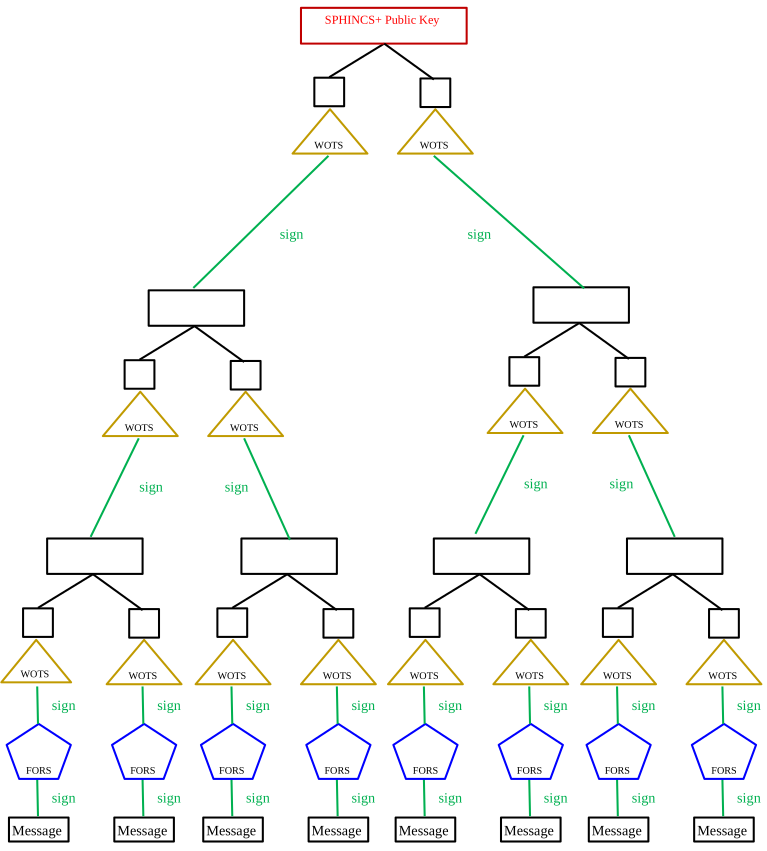
\includegraphics[width=1.1\linewidth]{fig/sphıncs.png}
        \caption{SPHINCS+ General structure}
        \label{fig:SPHINCS}
    \end{figure}
\end{section}


\begin{subsection}{SPHINCS+ Key Generation}

Key generation derives a full SPHINCS+ key pair from three seeds: the secret seed, the PRF key, and the public seed. It first initializes the ADRS value with a zero‐filled 32‐byte string and configures it for the top-level XMSS tree by setting the layer address to \(d-1\). The root node of that tree is computed via a single call to \texttt{xmss\_node}, which absorbs the secret seed, the public seed, and the ADRS state. Finally, the algorithm returns the secret key tuple \((\mathit{SK}.\mathit{seed},\,\mathit{SK}.\mathit{prf},\,\mathit{PK}.\mathit{seed},\,\mathit{PK}.\mathit{root})\) alongside the public key \((\mathit{PK}.\mathit{seed},\,\mathit{PK}.\mathit{root})\) (see Algorithm~\ref{alg:sphincs_keygen}).

\begin{algorithm}
\caption{SPHINCS\_keyGen -- Generate a SPHINCS+ key pair}
\label{alg:sphincs_keygen}

\textbf{Input:} None \\
\textbf{Output:} SPHINCS+ private key \texttt{SK}, SPHINCS+ public key \texttt{PK}

\vspace{0.3cm}

\begin{tabular}{ll}
1: & Generate uniformly random $n$-byte strings: \texttt{SK.SEED}, \texttt{SK.PRF}, \texttt{PK.SEED} \\
2: & Initialize \texttt{ADRS} as a zeroed address structure \\
3: & \texttt{PK.root} $\leftarrow$ \texttt{treehash(SK\_SEED, PUB\_SEED, ADRS)} \\
4: & \texttt{SK} $\leftarrow$ \texttt{SK.SEED $\parallel$ SK.PRF $\parallel$ PUB.SEED $\parallel$ PK.root} \\
5: & \texttt{PK} $\leftarrow$ \texttt{PK.SEED $\parallel$ PK.root} \\
6: & \textbf{return} \texttt{SK, PK}
\end{tabular}
\end{algorithm}

\end{subsection}

\begin{subsection}{SPHINCS+ Sign}

Signature generation begins by initializing the ADRS to zero and optionally randomizing the message randomizer input. The PRF keyed by \(\mathit{SK}.\mathit{prf}\) produces the randomness \(R\) that is prepended to the signature. A message digest is then computed over \(R\), the public seed, the root, and the message itself. This digest is split into the message digest bits \(\mathit{md}\) and the tree/leaf indices \(\mathit{idx\_tree},\mathit{idx\_leaf}\). The FORS scheme is applied at the lowest layer (layer 0) to sign \(\mathit{md}\), yielding \(\mathit{SIG\_FORS}\) and an authenticated public key \(\mathit{PK\_FORS}\). Finally, the hypertree (HT) signature over \(\mathit{PK\_FORS}\) is computed and appended, producing the full SPHINCS+ signature (see Algorithm~\ref{alg:spx_sign})

\begin{algorithm}
    \caption{spx\_sign -- Generating a SPHINCS+ signature}
    \label{alg:spx_sign}
    \textbf{Input:} Message \texttt{M}, private key \texttt{SK} = (\texttt{SK.seed}, \texttt{SK.prf}, \texttt{PK.seed}, \texttt{PK.root}) \\
    \textbf{Output:} SPHINCS+ signature \texttt{SIG}

    \vspace{0.2cm}

    \begin{tabular}{ll}
    1:  & \texttt{ADRS} $\leftarrow$ \texttt{toByte(0, 32)} \\
    2:  & \texttt{opt}  $\leftarrow$ \texttt{PK.seed} \\
    3:  & \textbf{if} \texttt{RANDOMIZE} \textbf{then} \\
    4:  & \quad \texttt{opt}  $\leftarrow$ \texttt{rand(n)} \\
    5:  & \textbf{end if} \\
    6:  & \texttt{R}    $\leftarrow$ \texttt{PRF\_msg(SK.prf, opt, M)} \\
    7:  & \texttt{SIG}  $\leftarrow$ \texttt{R} \\
    8:  & \texttt{digest} $\leftarrow$ \texttt{H\_msg(R, PK.seed, PK.root, M)} \\
    9:  & \texttt{tmp\_md}       $\leftarrow$ first $\lfloor(\mathit{ka}+7)/8\rfloor$ bytes of \texttt{digest} \\
    10: & \texttt{tmp\_idx\_tree} $\leftarrow$ next $\lfloor(h - h/d +7)/8\rfloor$ bytes of \texttt{digest} \\
    11: & \texttt{tmp\_idx\_leaf} $\leftarrow$ next $\lfloor(h/d +7)/8\rfloor$ bytes of \texttt{digest} \\
    12: & \texttt{md}      $\leftarrow$ first \texttt{ka} bits of \texttt{tmp\_md} \\
    13: & \texttt{idx\_tree} $\leftarrow$ first $(h - h/d)$ bits of \texttt{tmp\_idx\_tree} \\
    14: & \texttt{idx\_leaf} $\leftarrow$ first $h/d$ bits of \texttt{tmp\_idx\_leaf} \\
    15: & \texttt{ADRS.setLayerAddress(0)} \\
    16: & \texttt{ADRS.setTreeAddress(idx\_tree)} \\
    17: & \texttt{ADRS.setType(FORS\_TREE)} \\
    18: & \texttt{ADRS.setKeyPairAddress(idx\_leaf)} \\
    19: & \texttt{SIG\_FORS} $\leftarrow$ \texttt{fors\_sign(md, SK.seed, PK.seed, ADRS)} \\
    20: & \texttt{SIG}      $\leftarrow$ \texttt{SIG} \texttt{||} \texttt{SIG\_FORS} \\
    21: & \texttt{PK\_FORS} $\leftarrow$ \texttt{fors\_pkFromSig(SIG\_FORS, md, PK.seed, ADRS)} \\
    22: & \texttt{ADRS.setType(TREE)} \\
    23: & \texttt{SIG\_HT}   $\leftarrow$ \texttt{ht\_sign(PK\_FORS, SK.seed, PK.seed, idx\_tree, idx\_leaf)} \\
    24: & \texttt{SIG}      $\leftarrow$ \texttt{SIG} \texttt{||} \texttt{SIG\_HT} \\
    25: & \textbf{return} \texttt{SIG}
    \end{tabular}
\end{algorithm}



\begin{table}[ht]
  \centering
  \begin{tabular}{|l|}
    \hline
    \textbf{Signature}                         \\ \hline
    Randomness \(R\)                         \\ \hline
    FORS Signature \(\mathrm{SIG}_{\mathrm{FORS}}\)        \\ \hline
    HT Signature \(\mathrm{SIG}_{\mathrm{HT}}\)        \\ \hline
  \end{tabular}
  \caption{SPHINCS+ signature data format}
  \label{tab:slh-dsa-format}
\end{table}



\end{subsection}

\begin{subsection}{SPHINCS+ Verify}

Verification mirrors signing: it parses the incoming signature into \(R\), \(\mathit{SIG\_FORS}\), and \(\mathit{SIG\_HT}\). The verifier recomputes the message digest and splits it into \(\mathit{md}\), \(\mathit{idx\_tree}\), and \(\mathit{idx\_leaf}\). It then re-derives the FORS public key by running \(\mathit{fors\_pkFromSig}\) on \(\mathit{SIG\_FORS}\) and \(\mathit{md}\). Finally, the hypertree signature is checked with \(\mathit{ht\_verify}\), which returns \(\mathit{true}\) only if every component matches the stored public root (see Algorithm~\ref{alg:spx_verify}).

\begin{algorithm}
    \caption{spx\_verify -- Verify a SPHINCS+ signature SIG on a message M using a SPHINCS+ public key PK}
    \label{alg:spx_verify}
    \textbf{Input:} Message \texttt{M}, signature \texttt{SIG}, public key \texttt{PK} \\
    \textbf{Output:} Boolean

    \vspace{0.2cm}

    \begin{tabular}{ll}
        1:  & \texttt{ADRS} $\leftarrow$ \texttt{toByte(0, 32)} \\
        2:  & \texttt{R} $\leftarrow$ \texttt{SIG.getR()} \\
        3:  & \texttt{SIG\_FORS} $\leftarrow$ \texttt{SIG.getSIG\_FORS()} \\
        4:  & \texttt{SIG\_HT} $\leftarrow$ \texttt{SIG.getSIG\_HT()} \\
        5:  & \texttt{digest} $\leftarrow$ \texttt{H\_msg(R, PK.seed, PK.root, M)} \\
        6:  & \texttt{tmp\_md} $\leftarrow$ first $\lfloor(\mathit{ka}+7)/8\rfloor$ bytes of \texttt{digest} \\
        7:  & \texttt{tmp\_idx\_tree} $\leftarrow$ next $\lfloor(h - h/d +7)/8\rfloor$ bytes of \texttt{digest} \\
        8:  & \texttt{tmp\_idx\_leaf} $\leftarrow$ next $\lfloor(h/d +7)/8\rfloor$ bytes of \texttt{digest} \\
        9:  & \texttt{md} $\leftarrow$ first \texttt{ka} bits of \texttt{tmp\_md} \\
        10: & \texttt{idx\_tree} $\leftarrow$ first $(h - h/d)$ bits of \texttt{tmp\_idx\_tree} \\
        11: & \texttt{idx\_leaf} $\leftarrow$ first $h/d$ bits of \texttt{tmp\_idx\_leaf} \\
        12: & \texttt{ADRS.setLayerAddress(0)} \\
        13: & \texttt{ADRS.setTreeAddress(idx\_tree)} \\
        14: & \texttt{ADRS.setType(FORS\_TREE)} \\
        15: & \texttt{ADRS.setKeyPairAddress(idx\_leaf)} \\
        16: & \texttt{PK\_FORS} $\leftarrow$ \texttt{fors\_pkFromSig(SIG\_FORS, md, PK.seed, ADRS)} \\
        17: & \texttt{ADRS.setType(TREE)} \\
        18: & \textbf{return} \texttt{ht\_verify(PK\_FORS, SIG\_HT, PK.seed, idx\_tree, idx\_leaf, PK.root)} \\
    \end{tabular}
\end{algorithm}


\end{subsection}
